\chapter{Interpretability-performance trade-offs}\label{sec:exps2}


Now that we trained baseline policies and validated the proposed methodology, we use the latter to tackle open problems in interpretable reinforcement learning. For each environment, we fix the imitation learning algorithm and save the best baseline policy of each class in terms of episodic rewards after unfolding them. Each single Python policy is then \textbf{run again on the same dedicated CPU} for 100 new environment episodes (similarly to choosing a classifier with validation score and reporting the test score in the context of supervised learning).
\begin{figure}
    \centering
    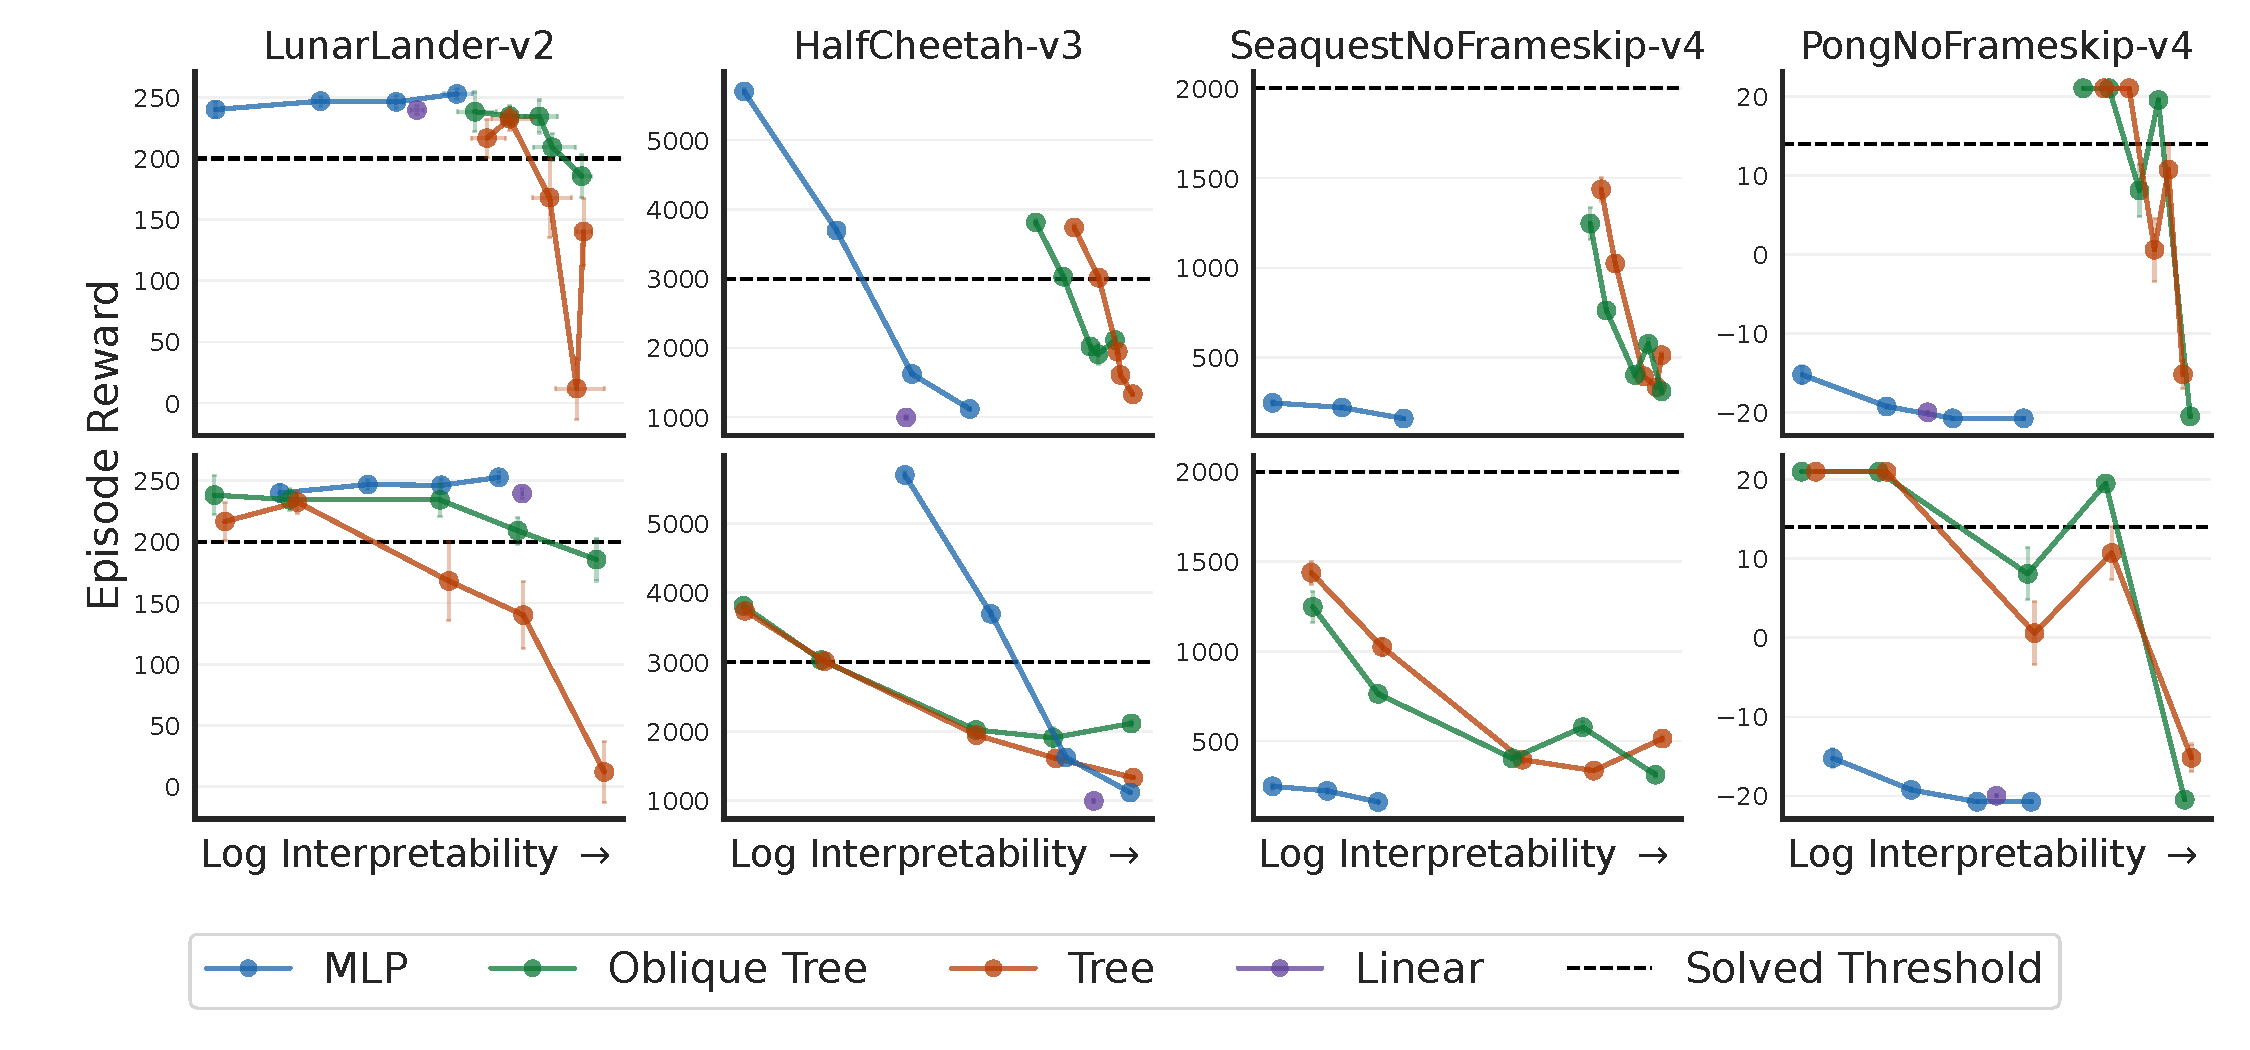
\includegraphics[trim={1.4cm 0 0 0},clip,width=1\textwidth]{images/images_part3/trade_off_select_combine_one_plot.pdf}
    \caption{Interpretabality-Performance trade-offs. Top row, interpretability is measured with step inference times. Bottom row, the interpretability is measured with policy size. We plot 95\% bootstrapped confidence intervals around means on both axes.}
    \label{fig:trade-off-summary}
\end{figure}

\paragraph{Is it possible to compute interpretable policies for high-dimensional environments?} \cite{glanois-survey} claim that computing an interpretable policy for high dimensional MDPs is difficult since it is similar to program synthesis which is known to be NP-hard \cite{program-synth}. Using our measures of interpretability, we can corroborate this claim. On Figure \ref{fig:trade-off-summary}, we can indeed observe that some relatively interpretable policies can solve Pong (20 state dimensions) or HalfCheetah (17 state dimensions) while for very high-dimensional environments like Seaquest (180 state dimensions), no baseline can solve the game.


\paragraph{For what environment are there good interpretable policies?}
We fitted a random forest regressor \cite{random} to predict the interpretability values of our baseline policies using environment attributes. In Table \ref{tab:combined_importance} we report the importance of each environment attribute when it comes to accurately predicting interpretability scores. We show that as hinted previously, the states dimensions of the environment is determining to predict the interpretability of good policies. Unsurprisingly, expert attributes also influence interpretability: for the environments where there is a positive large gap between expert and threshold rewards, the task could be considered easy and vice-versa.

\begin{table}
\centering
\small
\begin{tabular}{lcc}
\toprule
Environment Attributes & Importance for Step inference & Importance for Policy size \\
\midrule
States dimension & \textbf{80.87} & \textbf{35.52} \\
Expert episodes lengths & 11.39 & 9.28 \\
Episode reward of random & 2.26 & 4.75 \\
Expert episode reward & 1.51 & 16.80 \\
Episode reward to solve & 1.41 & 14.26 \\
Actions dimension & 1.41 & 2.02 \\
Expert reward - Solve reward & 1.15 & 17.37 \\
\bottomrule
\end{tabular}
\caption{Environment attributes importance to predict interpretability using either of our metrics.}
\label{tab:combined_importance}
\end{table}

\paragraph{How does interpretability influence performance?}
\cite{empirical-evidence,theory1} show the existence of linear and tree policies respectively that solve MuJoCo and continuous maze environments respectively; essentially showing that there exist environments for which policies more interpretable than deep neural networks can still compete performance-wise. Our evaluation indeed shows the existence of such environments. On Figure \ref{fig:trade-off-summary} we observe that on, e.g., 
LunarLander, increasing policy interpretability up to a certain point does not decrease reward. Actually, we can observe that for Pong a minimum level of interpretability is required to solve the game. Indeed, as stated in \cite{study-0}, optimizing interpretability can also be seen as regularizing the policy which can increase generalization capabilities. 
The key observation is that the policy class achieving the best interpretability-performance trade-off depends on the problem. Indeed, independent of the interpretability proxy metric, we see on Figure \ref{fig:trade-off-summary} that for LunarLander it is an MLP that achieves the best trade-off while for Pong it is a tree. Next, we compare our proxies for interpretability with another one; the verification time of policies used in \cite{viper,lens-complexity}.


\subsection{Verifying interpretable policies}
\cite{lens-complexity} states that the cost of formally verifying properties of MLPs scales exponentially with the number of the parameters. Hence, they propose to measure interpretability of a policy as the computations required to verify properties of actions given state subspaces, what they call local explainability queries \cite{query}. Before \cite{lens-complexity}, \cite{viper} also compared the time to formally verified properties of trees to the time to verify properties of MLPs to evaluate interpretability. In practice, this amounts to passing states and actions bounds and solving the SAT problem of finding a state in the state bounds for which the policy outputs an action in the action bounds. For example, for the LunarLander problem, a query could be to verify if when the y-position of the lander is below some threshold value, i.e, when the lander is close to the ground, there exists a state such that the tested policy would output the action of pushing towards the ground: if the solver outputs ``SAT'', then there is a risk that the lander crashes. 

Designing interesting queries covering all risks is an open problem, hence to evaluate the verification times of our baseline policies, we generate 500 random queries per environment by sampling state and action subspaces uniformily. Out of those queries we only report the verification times of ``UNSAT'' queries since to verify that, e.g., the lander does not crash we want the queries mentioned above to be ``UNSAT''. We also only verify instances of ReLU MLPs using \cite{maraboupy} for this experiment as verifying decision trees requires a different software \cite{z3} for which verification times would not be comparable.
\begin{figure}[ht]
    \centering
    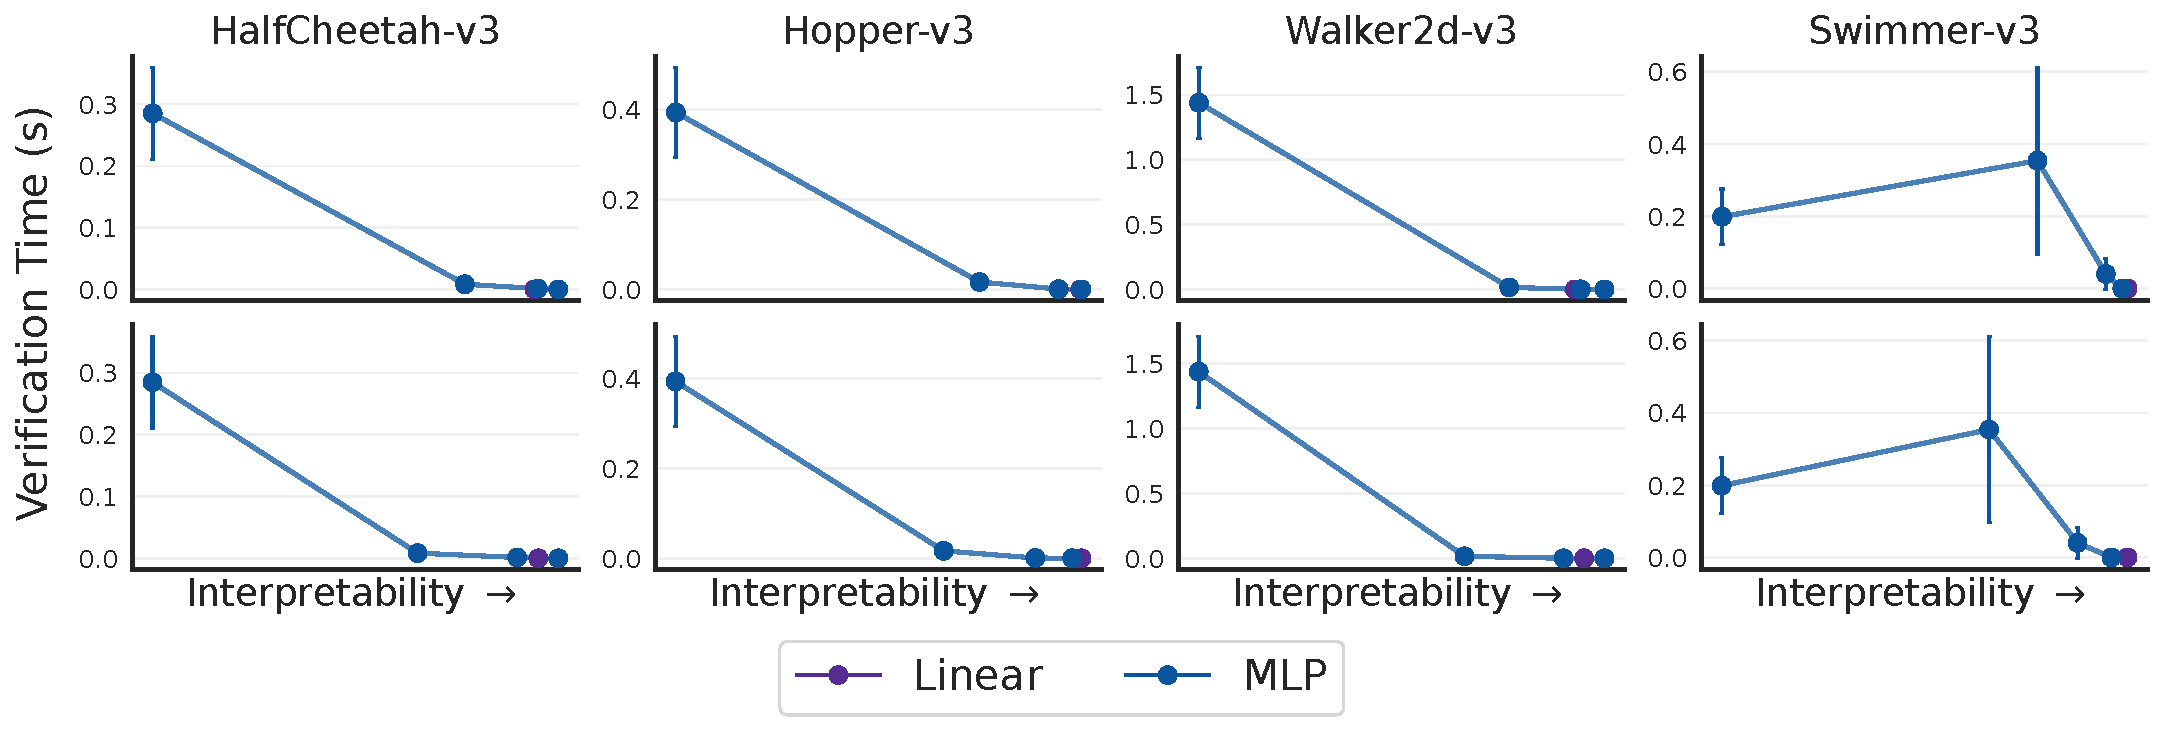
\includegraphics[width=1\linewidth]{images/images_part3/verification_tradeoff.pdf}
    \caption{Verification time as a function of policy interpretability. Top row, interpretability is measured with step inference times. Bottom row, the interpretability is measured with policy size. We plot 95\% confidence intervals around means on both axes.}
    \label{fig:trade-off-verif}
\end{figure}

On Figure \ref{fig:trade-off-verif}, we can observe that verification time decreases exponentially with MLP interpretability, both memory and inference speed, as shown in \cite{lens-complexity}. This is another good validation of our proposed methodology as well as a motivation to learn interpretable policies. 

\section{Experimental details}

In this section we give all the experimental details necessary to reproduce our results.



\begin{table}[ht]
\centering
\small
\begin{tabular}{lll}
\hline
\textbf{Classic} & \textbf{MuJoCo} & \textbf{OCAtari}\\
\hline
CartPole (4, 2, \textbf{490}) & Swimmer (8, 2, \textbf{300}) & Breakout (452, 4, \textbf{30})\\
LunarLander (8, 4, \textbf{200}) & Walker2d (17, 6, \textbf{2000}) & Pong (20, 6, \textbf{14})\\
LunarLanderContinuous (8, 2, \textbf{200}) & HalfCheetah (17, 6, \textbf{3000}) & SpaceInvaders (188, 6, \textbf{680})\\
BipedalWalker (24, 4, \textbf{250}) & Hopper (11, 3, \textbf{2000}) & Seaquest (180, 18, \textbf{2000})\\
MountainCar (2, 3, \textbf{90}) & \\
MountainCarContinuous (2, 1, \textbf{-110}) & \\
Acrobot (6, 3, \textbf{-100}) & \\
Pendulum (3, 1, \textbf{-400}) & \\
\hline
\end{tabular}
\caption{Summary of considered environments (dimensions of states and number or dimensions of actions, \textbf{reward thresholds}). The rewards thresholds are obtained from gymnasium \cite{gymnasium}. For OCAtari environments, we choose the thresholds as the minimum between the DQN expert from \cite{zoo} and the human scores. We also adapt subjectively some thresholds that we find too restrictive especially for MuJoCo (for example, the PPO expert from \cite{zoo} has 2200 reward on Hopper while the default threshold was 3800).}
\label{tab:envs}
\end{table}

\begin{table}
    \centering
    \footnotesize
    \begin{tabular}{c|cccccc}
    \toprule
    Envs & BC & BC & DAgger & DAgger & $Q$ & $Q$-DAgger\\
     & 50K & 100K & 50K & 100K & 50K & 100K\\
    \midrule
    Classic& 50 (PPO, DQN)& 50 (PPO, DQN)& 50 (PPO, DQN)& 50 (PPO, DQN)&  50 (DQN) & 50 (DQN)\\
    OCAtari& 0 & 0 & 0 & 5 (DQN)&  0 & 5 (DQN)\\
    Mujoco& 10 (SAC)& 10 (SAC)& 10 (SAC)& 10 (SAC)&  0 & 0\\
    \bottomrule
    \end{tabular}
    \caption{Repetitions of each imitation learning algorithm on each environment. We specify which deep reinforcement learning agent from the zoo~\cite{zoo} uses as experts in parentheses.}
    \label{tab:repet-distill}
\end{table}

\section{All interpretability-performance trade-offs}
In this appendix we provide the interpretability-performance trade-offs of all the tested environments. All the measures come from the experiment from Section \ref{sec:res-trade-offs}.

\begin{figure}
    \centering
    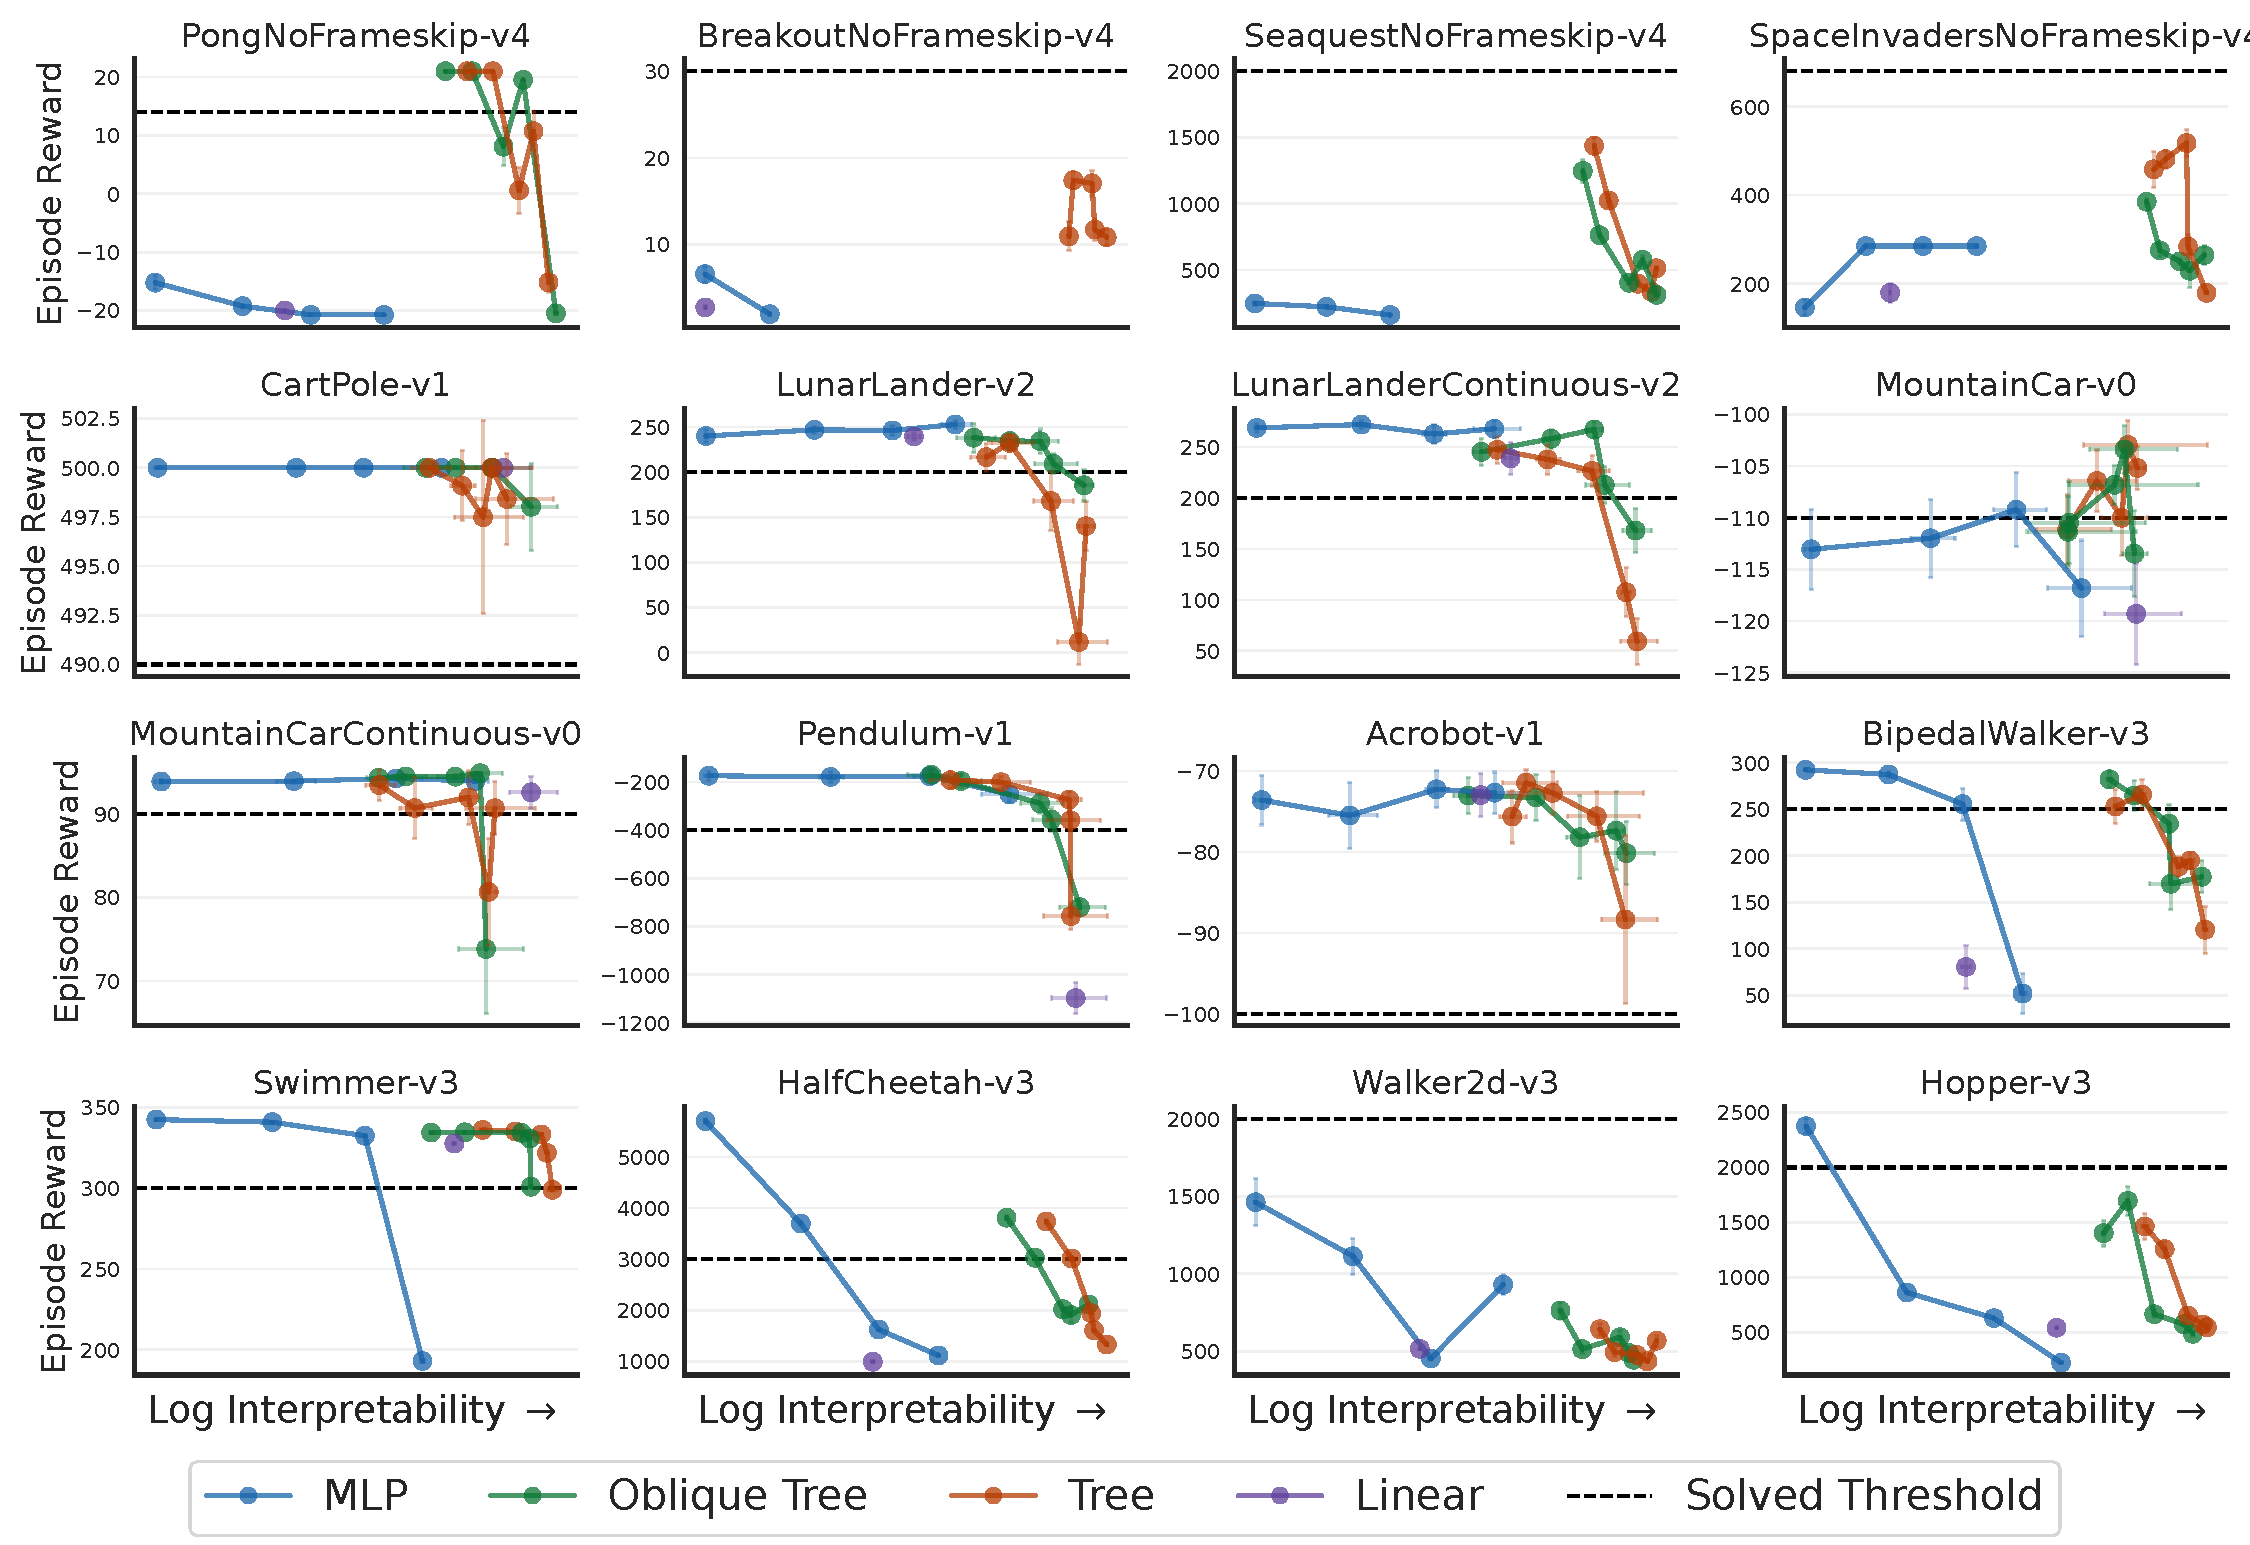
\includegraphics[width=1\linewidth]{images/images_part3/trade_off_step_times.pdf}
    \caption{Trade-off Cumulative Reward vs. Step Inference Time}
    \label{fig:trade-off}
\end{figure}

\begin{figure}[ht]
    \centering
    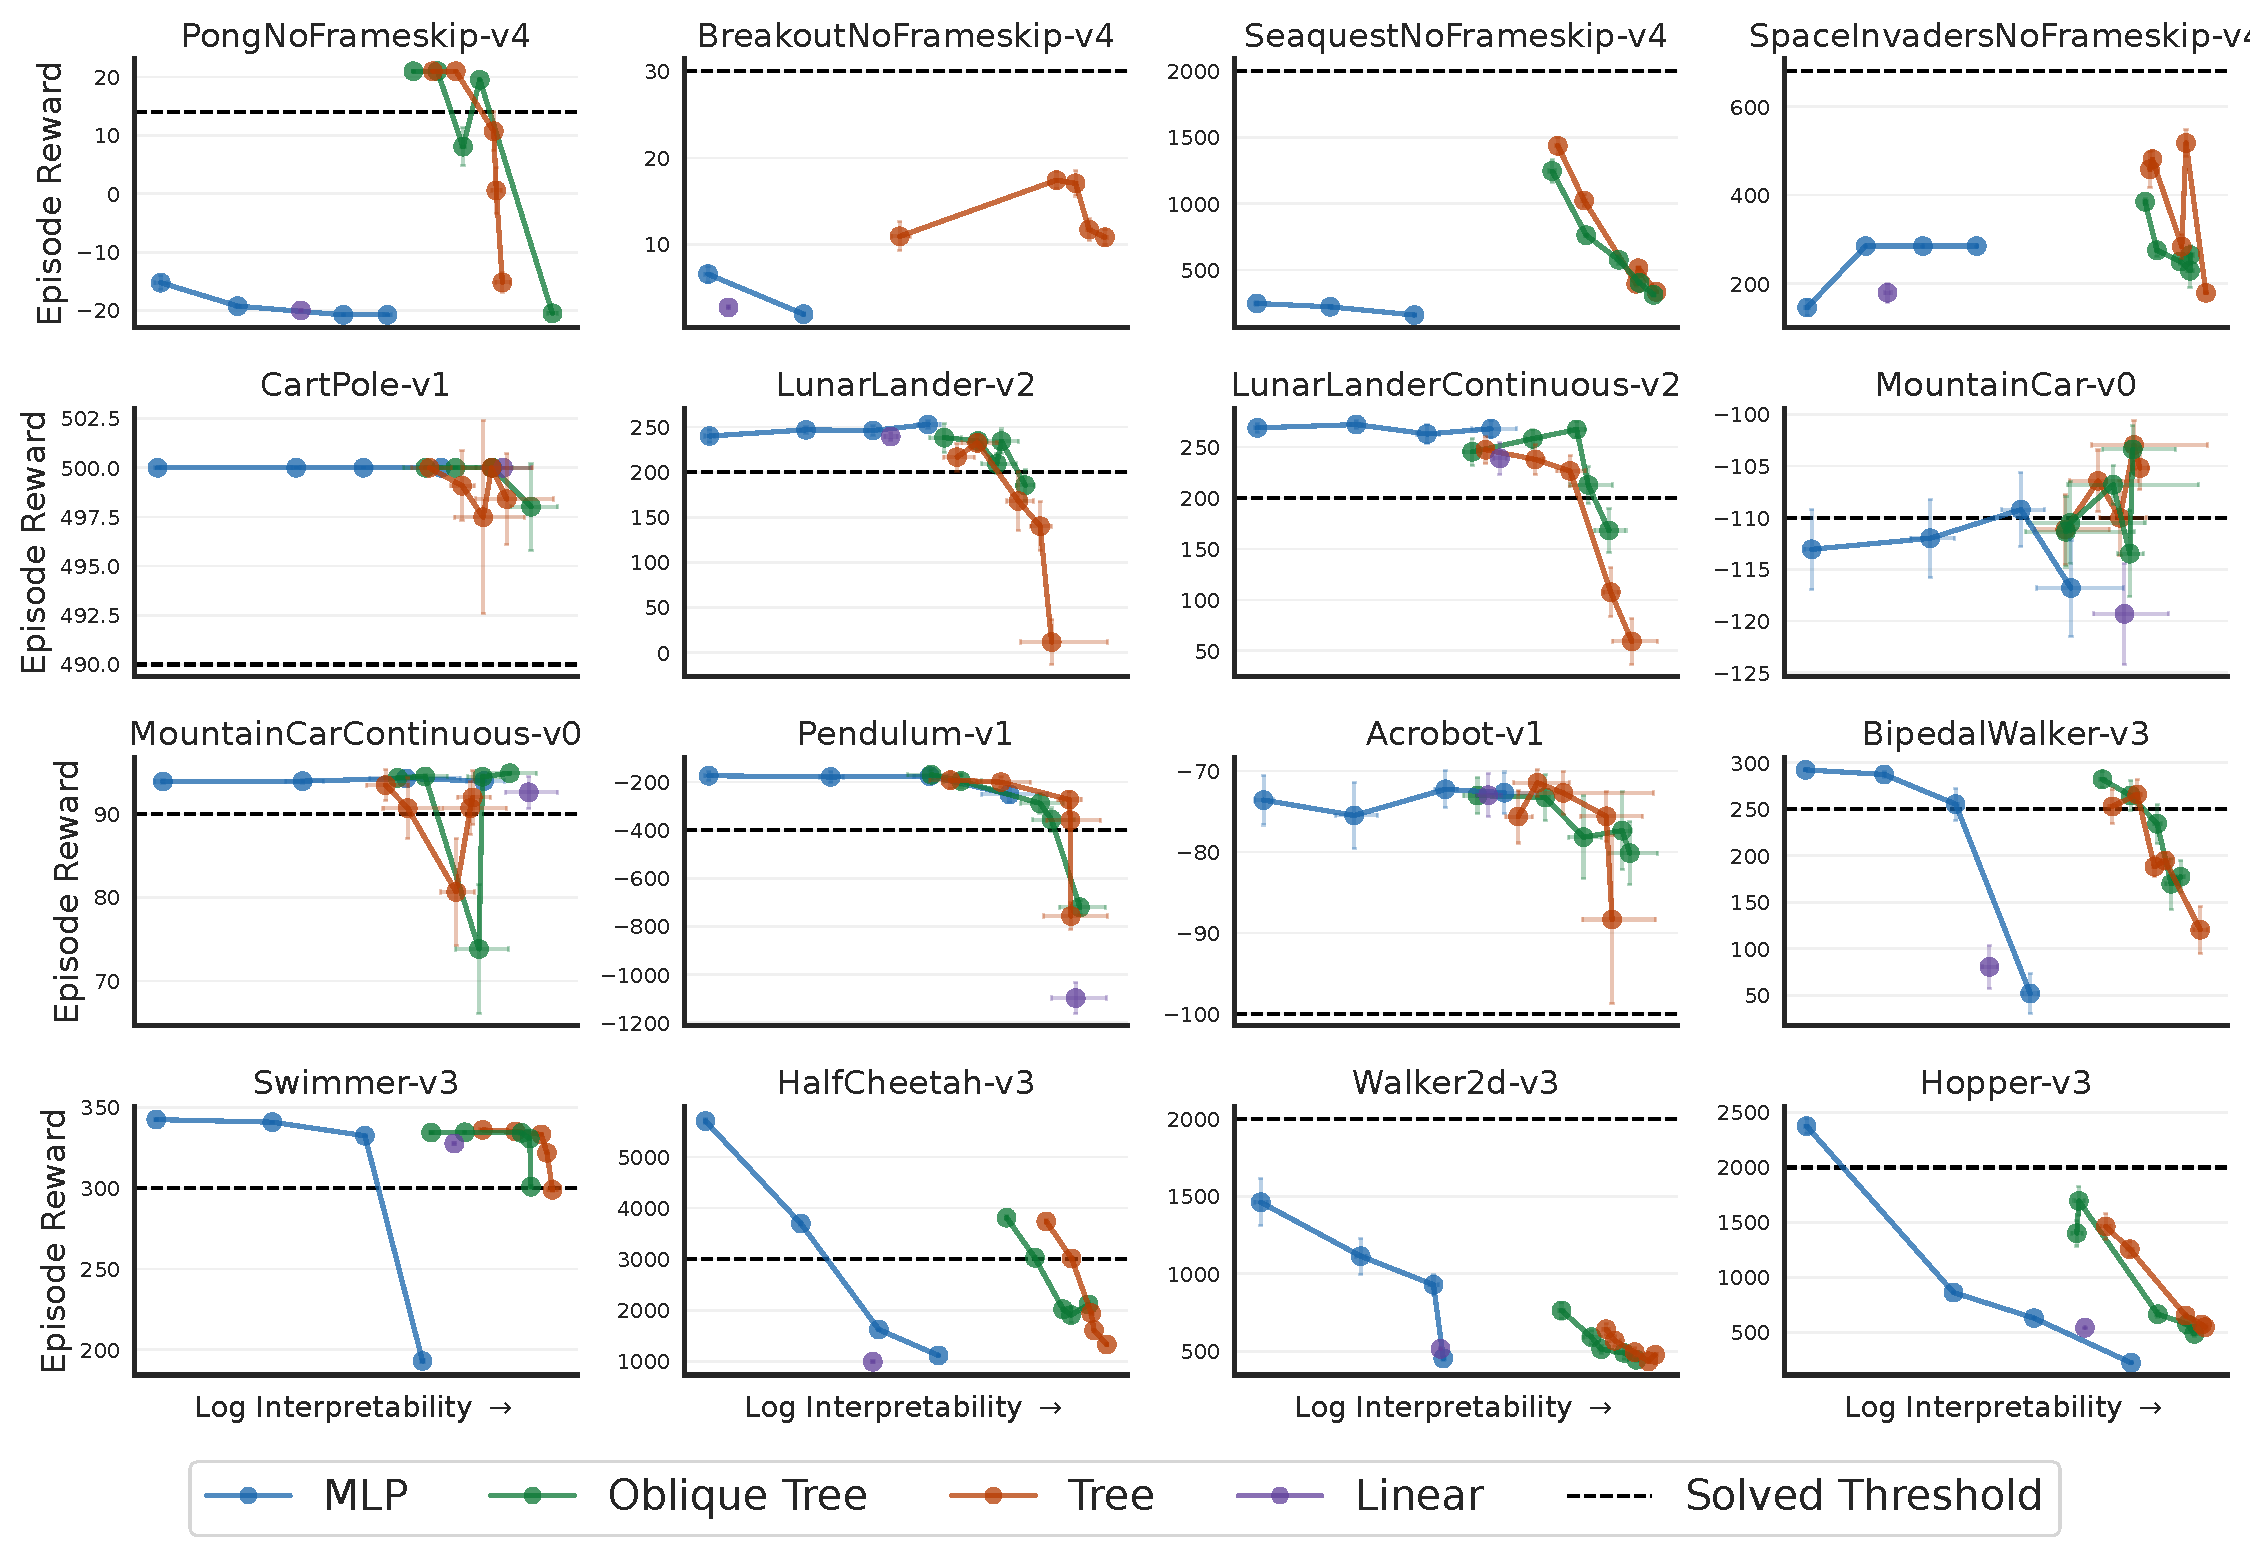
\includegraphics[width=0.95\linewidth]{images/images_part3/trade_off.pdf}
    \caption{Trade-off Cumulative Reward vs. Episode Inference Time}
    \label{fig:trade-off-episode}
\end{figure}

\begin{figure}[ht]
    \centering
    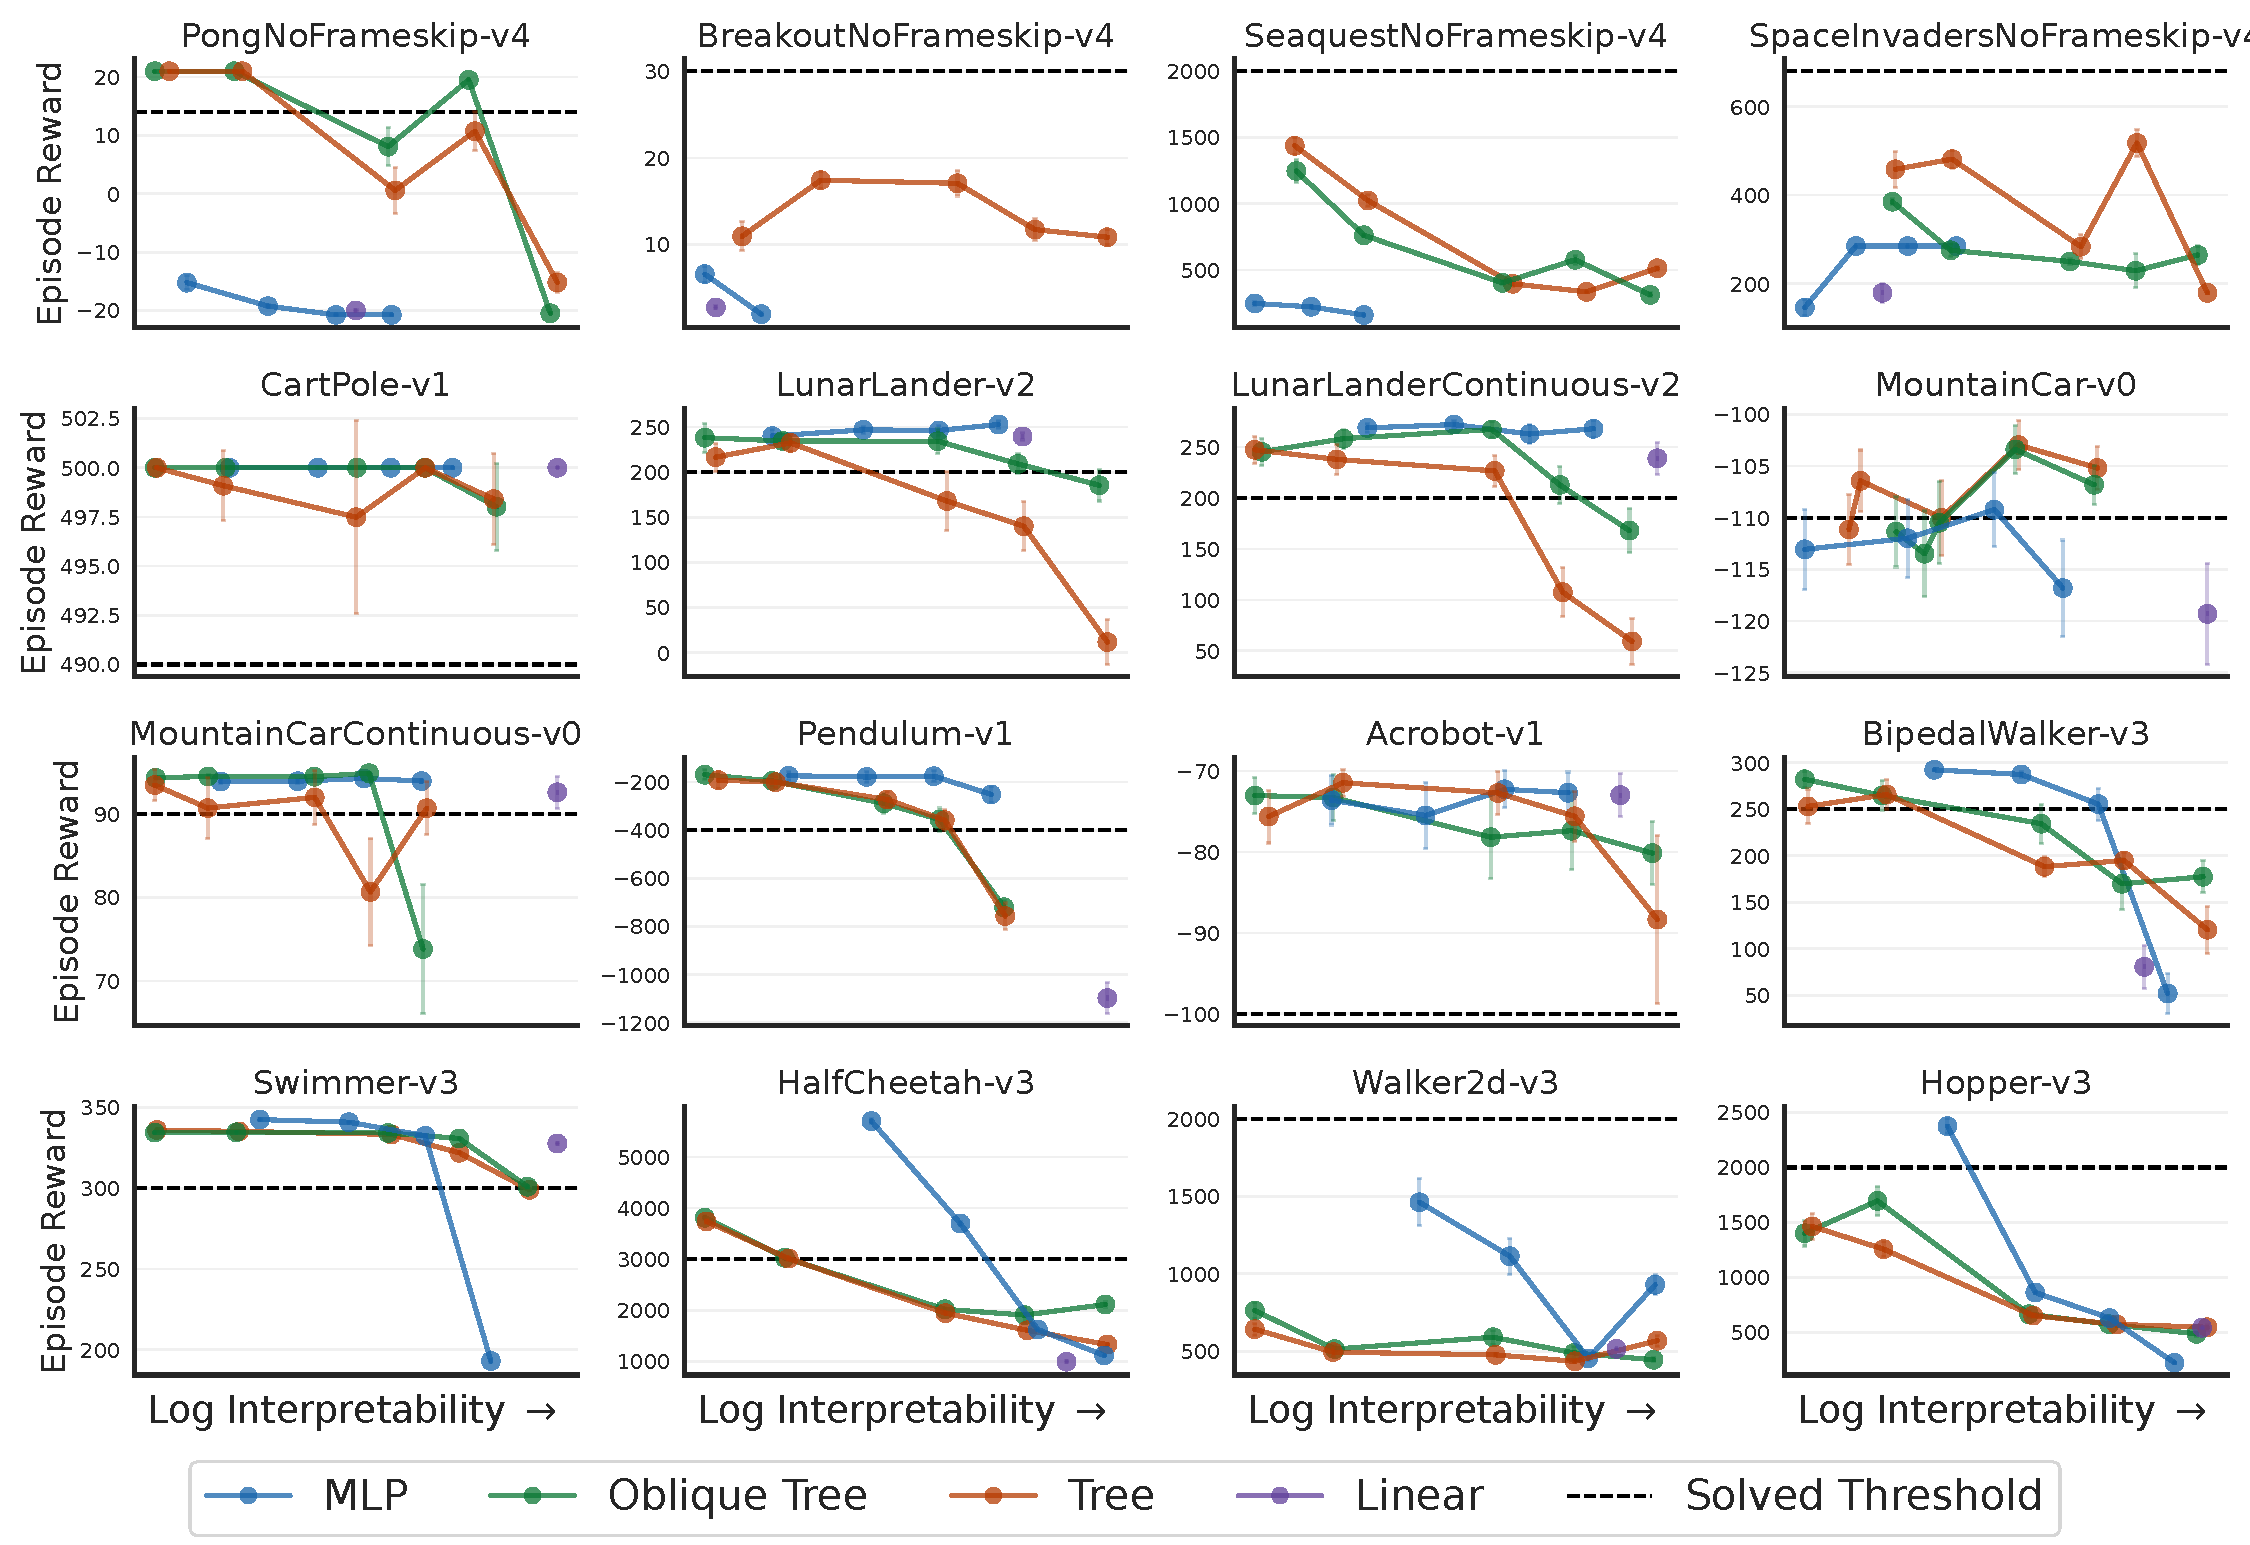
\includegraphics[width=0.95\linewidth]{images/images_part3/trade_off_size.pdf}
    \caption{Trade-off Cumulative Reward vs. Policy Size}
    \label{fig:trade-off-size}
\end{figure}
\section{Limitations and conclusions}\label{sec:ccl}
We have shown that our proposed methodology provides researchers with a sound way of evaluating policy interpretability. In particular, we have shown that unfolding policies in a common language such as Python is a key component of our methodology to ensure that interpretability depends on the policy complexity (c.f. Figure \ref{fig:abl-proxies}). Furthermore, we were able to show that the proxies we use for interpretability leads to similar conclusions from user studies of interpretability or from other empirical evaluations of interpretability (c.f. Figures \ref{fig:abl-proxies}, \ref{fig:trade-off-summary}, and \ref{fig:trade-off-verif}). Using the proposed methodology, we were able to illustrate the trade-offs between episodic reward and interpretability of policies from different classes (c.f. Figure \ref{fig:trade-off-summary}) and showed the crucial need of our methodology as there is no better off policy class across tasks and metrics (c.f. Figures \ref{fig:perf-combined}, \ref{fig:abl-proxies}, and \ref{fig:trade-off-summary}). 

A nice property of our methodology is that it is independent of the learning algorithm of the interpretable policy. We chose imitation learning but it could have been a random search in the policies parameters space \cite{empirical-evidence}. Furhtermore, there sould be no limitation to use our methodology to evaluate the interpretability of arbitrary compositions of linear policies, trees and oblique trees, and MLPs, such as the hybrid policies from \cite{shindo2024blendrl}. However, the unfolded version of policies with loops which lengths depend on the state would change between step, hence, the policy size metric value will change during episodes. This is not necessarily a strong limitation but would require more work on the unfolding procedures as well as on defining episodic metrics. 

In the future, it would be interesting to compare episodic to averaged measures of interpretability. Indeed, we additionally show in Appendix \ref{fig:trade-off-episode} the interpretability-performance trade-offs using the inference time summed over entire episodes as the measure of interpretability. Even though using episodic inference does not change the trade-offs compared to step inference time, it is important to discuss this nuance in future work since a key difference between supervised learning and reinforcement learning interpretability could be that human operators would read policies multiple times until the end of a decision process. Using episodic metrics for interpretability is not as straightforward as someone would think as for some MDPs, e.g. Acrobot, the episodes lengths depend on the policy. We also did not evaluate the role of sparsity in the interpretability of linear and MLP policies even thought this could greatly influence the inference time. In the future it would be interesting to apply our methodologies to policies obtained with e.g. \cite{sparsity}. Moving away from evaluation, we also believe that our interpretable baselines can be used to train hierarchical agents \cite{hierarchical} using our baselines as options. We hope that our methodology as well as the provided baselines will pave the way to a more rigorous science of interpretable reinforcemeent learning.
